\documentclass{article}

\usepackage{url} 
\usepackage{geometry,afterpage}
\usepackage{pdfpages}
\usepackage{lastpage}
\usepackage{fancyhdr}
\usepackage{ngerman}
\usepackage{listings}

\usepackage{floatrow}
\usepackage[tableposition=top]{caption}
\floatsetup[table]{capposition=top}

\usepackage{amsmath, amssymb}

\usepackage[utf8]{inputenc}


\usepackage[numbib]{tocbibind}



\newcommand\twodigits[1]{%
   \ifnum#1<10 0#1\else #1\fi
}



\lhead{Elektronenbeugung}
\rhead{28.05.2021\\ J. Winkler}
%\cfoot{\twodigits{\thepage}~/ \pageref{LastPage}}
\cfoot{{\thepage}~/ \pageref{LastPage}}


\newcommand{\Ekin}{E_\text{kin}}

\begin{document}

\parindent0cm

\renewcommand{\max}{\operatorname{max}}
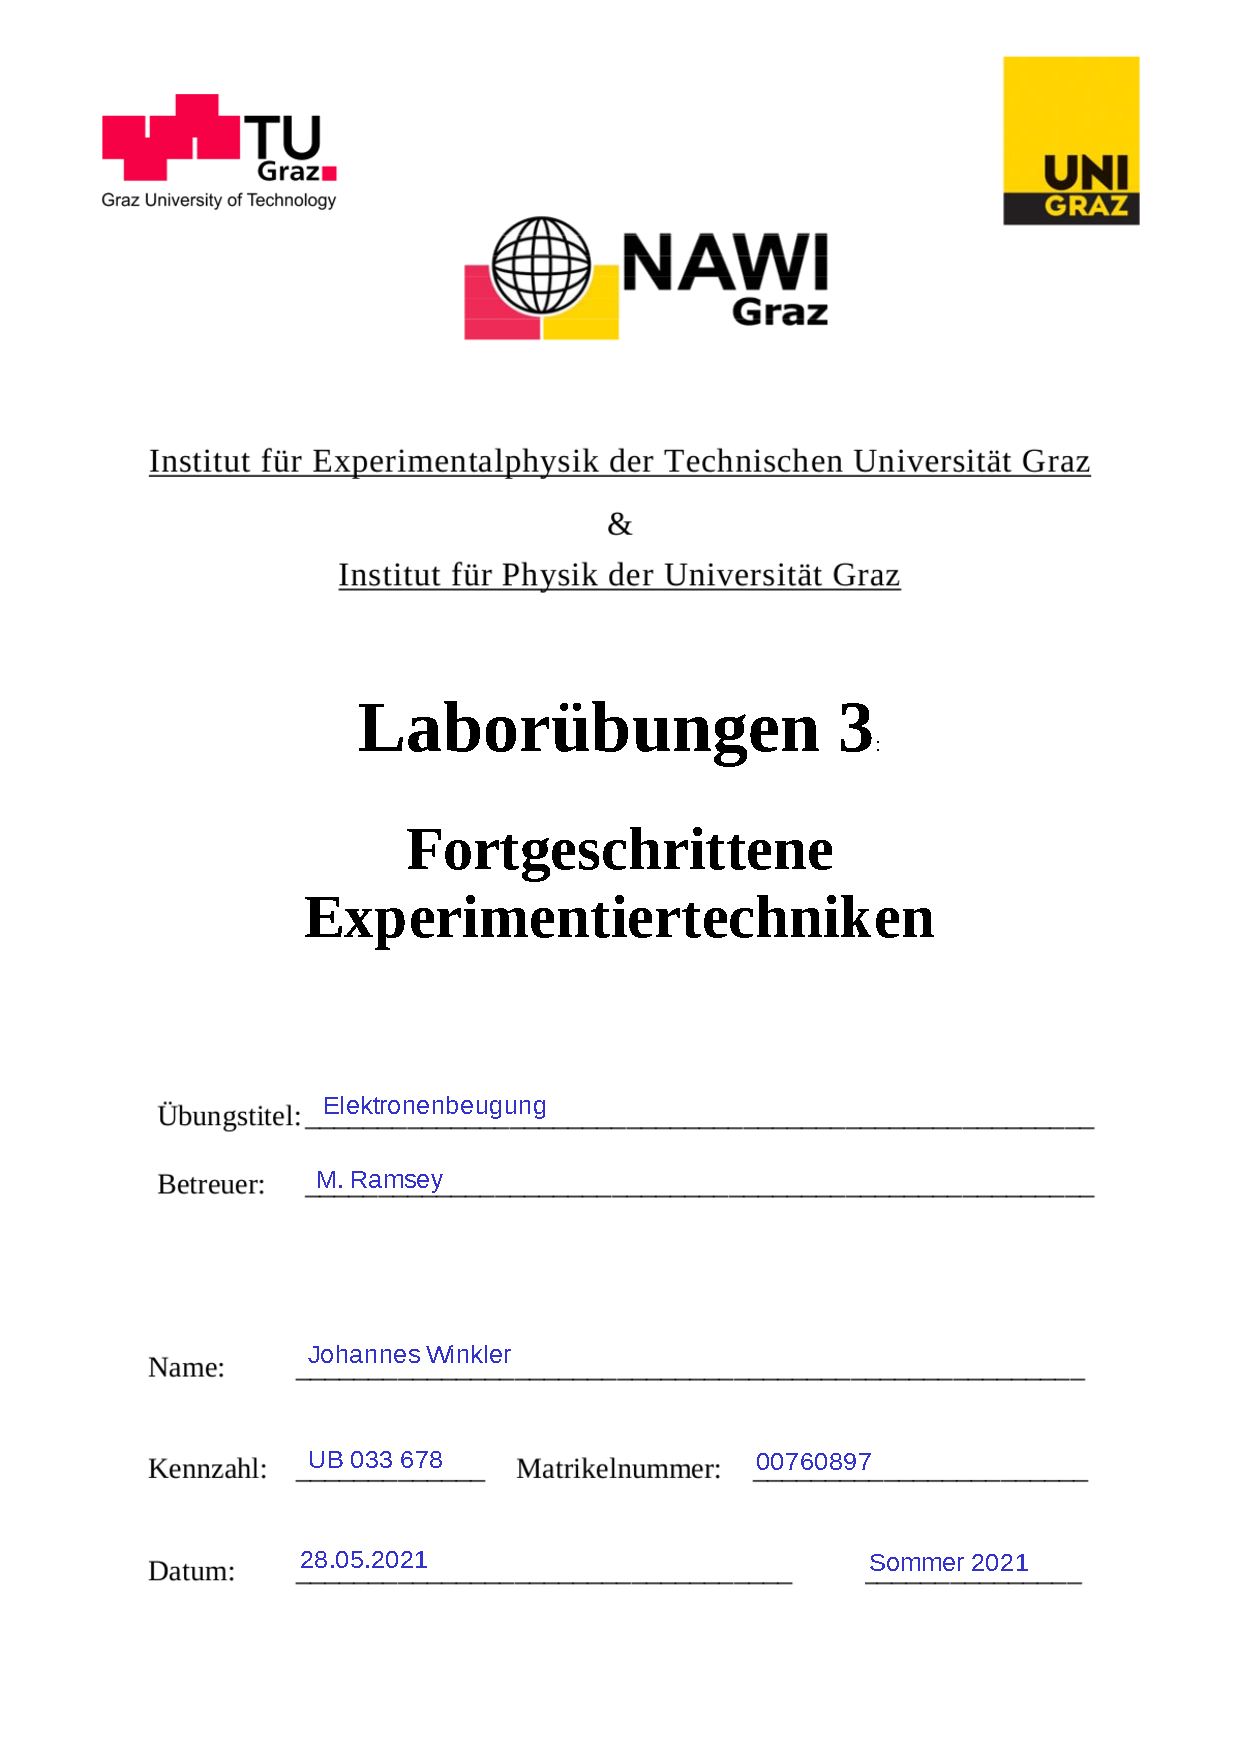
\includepdf{Deckblatt_neu_custom.pdf}

\tableofcontents
\newpage

\pagestyle{fancy}

\section{Aufgabenstellung}

\begin{enumerate}
\item Beugung von Elektronen an einer polykristalinen Graphitprobe
\begin{enumerate}
\item Berechnen Sie die Wellenlänge der Elektronen für die im Versuch
verwendeten Anoden- (Beschleunigungs-) spannungen; d.h. für den Bereich
zwischen 2~keV und 5~keV.
\item Die beobachteten Beugungsringe entsprechen den Abständen zweier
verschiedener Gitterebenen. Bestimmen Sie aus dem Durchmesser der
Beugungsringe den jeweiligen Gitterabstand. Dabei sind bei mind. 10
Elektronenenergien Messungen durchzuführen. 
\end{enumerate}
\item Aus dem Krümmungsradius der Elektronenbahn in einem homogenen
Magnetfeld ist die spezifische Ladung 	des Elektrons zu
bestimmen.
\begin{enumerate}
\item  Die Auslenkung des Elektronenstahls auf dem Leuchtschirm einer
Oszillographenröhre ist in Abhängigkeit von der Stärke des Stromes ($I_{\max}=2~$~A) durch die magnetfelderzeugenden Helmholzspulen bei zwei unterschiedlichen Anodenspannungen $U_A$ zu messen.	
\item Aus der Auslenkung ist der Krümmungsradius $r$ der Elektronenbahn, aus dem Spulenstrom ist die magnetische Induktion $B$ zu berechnen.
\item $\frac{1}{r}$ ist als Funktion der Induktion $B$ graphisch darzustellen. Die spezifische
Elektronenladung $\frac{e}{m_e}$ ist durch lineare Regression zu bestimmen. 
\end{enumerate}
\end{enumerate}


%\begin{figure}[H]
%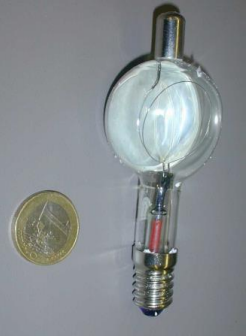
\includegraphics[scale=1.4]{versuch3.png}
%\caption{Vakuum Photozelle. Quelle: \cite{moodle}}
%\end{figure}

\section{Grundlagen}

Nach dem Wellen-Teilchen-Dualismus besitzen Elektronen sowohl eine Wellenlänge $\lambda$, als auch einen Impuls $p$. Nach de Broglie gilt zwischen den Größen folgender Zusammenhang
\begin{align}
\lambda = \frac{h}{p}
\label{eq:debroglie}
\end{align}
wobei $h=6.62607015\cdot 10^{-34}$~Js das Planck'sche Wirkungsquantum ist. Zusätzlich weiß man, dass sich der Impuls mit Hilfe der kinetischen Energie ausdrücken lässt
\begin{align*}
\frac{1}{2}\cdot m_e \cdot v^2 = \frac{p^2}{2\cdot m_e} = e\cdot U
\end{align*}
Mit $e=1.602176634\cdot 10^{-19}$~C und $m_e=9.1093837015\cdot 10^{-31}$~kg ist. Daraus folgt unmittelbar der Zusammenhang
\begin{align}
\lambda  &= \frac{h}{\sqrt{2\cdot m_e \cdot e\cdot U}} 
\label{eq:lambda}
\end{align}
% (inkl. Fehlerrechnung)
%\begin{align}
%\lambda \pm \Delta\lambda &= \frac{h}{\sqrt{2\cdot m_e \cdot e\cdot U}} \pm \frac{h}{\sqrt{2\cdot e}}\cdot \left(\frac{\Delta m_e}{2\cdot m_e \cdot \sqrt{m_e}} \cdot \frac{1}{\sqrt{U}} + \frac{1}{\sqrt{m_e}} \cdot \frac{\Delta U}{2\cdot U\cdot \sqrt{U}} \right) \\
%\lambda \pm \Delta\lambda &= \frac{h}{\sqrt{2\cdot m_e \cdot e\cdot U}} \pm \frac{h}{\sqrt{2\cdot m_e\cdot e \cdot U}}\cdot \left(\frac{\Delta m_e}{2\cdot m_e} +  \frac{\Delta U}{2\cdot U} \right)\\
%\lambda \pm \Delta\lambda &= \frac{h}{\sqrt{2\cdot m_e \cdot e\cdot U}}  \cdot \left[1 \pm  \left(\frac{\Delta m_e}{2\cdot m_e} +  \frac{\Delta U}{2\cdot U}\right) \right]
%\label{eq:lambda}
%\end{align}

%\begin{figure}[H]
%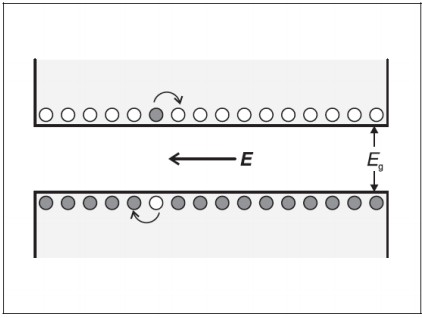
\includegraphics[scale=1.4]{bandabstand.png}
%\caption{Veranschaulichung des Bändermodells. Quelle: \cite{moodle}}
%\label{fig:bandabstand}
%\end{figure}


Die Elektronen werden gemäß der Bragg-Bedingung gebeugt.
\begin{align*}
n\cdot\lambda = 2\cdot d\cdot\sin(\vartheta)
\end{align*}
Dieser Zusammenhang ist in Grafik~\ref{fig:bragg} gegeben

\begin{figure}[H]
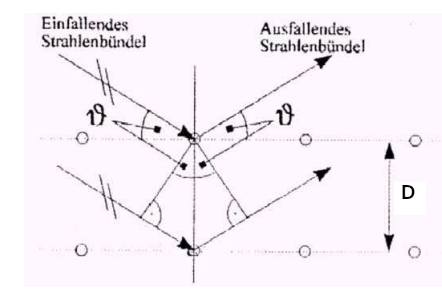
\includegraphics[scale=1.79]{bragg.png}
\caption{Visualisierung der Bragg-Bedingung. Quelle: \cite{moodle}}
\label{fig:bragg}

\end{figure}

Durch diverse Umformungen in \cite{moodle} folgt nun 
\begin{align}
D = \frac{2\cdot R}{r}\cdot n\cdot \lambda
\label{eq:gitterabstand}
\end{align}
wobei $D$ der Gitterabstand, $R=67.5~$mm der Radius der Glaskugel, $n=1$ die Beugungsordnung und $\lambda$ die Wellenlänge ist. Für die beiden Beugungsringe kann dadurch der Gitterabstand berechnet werden. Grafik~\ref{fig:gitterabst} zeigt die erwarteten Ergebnisse.

\begin{figure}[H]
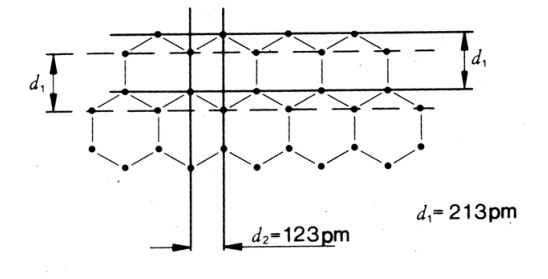
\includegraphics[scale=2.]{gitterabstand.png}
\caption{Gitterabstand des Graphitgitters mit den erwarteten Ergebnissen. Quelle: \cite{moodle}}
\label{fig:gitterabst}
\end{figure}


Für den zweiten Teil des Versuchs sind weitere Formeln nötig. Aus der Lorentzkraft $F=e\cdot v \cdot B$ (Vektoren stehen orthogonal) und der Zentrifugalkraft ergibt sich insgesamt
\begin{align*}
-e\cdot v \cdot B = \frac{m_e\cdot v^2}{r}
\end{align*}
Und daraus folgt
\begin{align*}
e_\text{spez} = -\frac{e}{m_e} = \frac{v}{r\cdot B}
\end{align*}
wobei $r$ der Krümmungsradius ist. Die kinetische Energie liefert zusätzlich $-e\cdot U = \frac{1}{2}m_e\cdot v^2$. Insgesamt lässt sich dadurch $v$ eliminieren.
\begin{align*}
e_\text{spez}^2 = \frac{v^2}{r^2\cdot B^2} =  \frac{-2\cdot e\cdot U}{m_e} \cdot \frac{1}{r^2\cdot B^2} = e_\text{spez}\cdot 2\cdot U \cdot \frac{1}{r^2\cdot B^2}
\end{align*}
Daraus folgt
\begin{align}
e_\text{spez} = \frac{2\cdot U}{r^2\cdot B^2}
\label{eq:espez}
\end{align}

Der Krümmungsradius kann durch geometrische Überlegungen berechnet werden. Dazu dient Skizze~\ref{fig:radius} als Veranschaulichung. Aus dem Satz von Thales folgt ein rechter Winkel und dadurch kann der Satz des Pythagoras angewendet werden.
\begin{align*}
\ell = \sqrt{d^2-s^2}
\end{align*}
Aus der Trigonometrie ergibt sich
\begin{align*}
\tan(\alpha) = \frac{s}{\ell}
\end{align*}
Letztendlich ergibt sich der Krümmungsradius durch
\begin{align*}
r = \frac{d}{2} \big / \tan(\alpha) = \frac{d\cdot \ell}{2\cdot s}
\end{align*}
\begin{align}
r = \frac{d\cdot \sqrt{d^2-s^2}}{2\cdot s}
\label{eq:radius}
\end{align}

\begin{figure}[H]
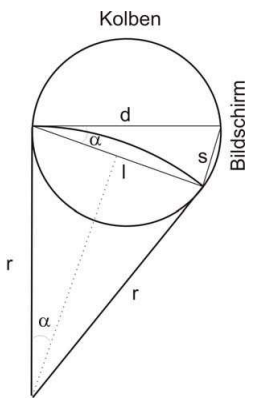
\includegraphics[scale=1.79]{radius.png}
\caption{Bestimmung des Krümmungsradius. Quelle: \cite{moodle}}
\label{fig:radius}

\end{figure}

Nach \cite{moodle} ist die magnetische Feldstärke zwischen den Helmholtz-Spulen räumlich konstant und gegeben durch
\begin{align}
B = \mu_0 \cdot \frac{n\cdot R^2}{(R^2+a^2)^{3/2}}\cdot I = \mu_0 \cdot 3367.255~\text{m}^{-1}\cdot I
\label{eq:Bfeld}
\end{align}

\section{Versuchsaufbau}

\begin{figure}[H]
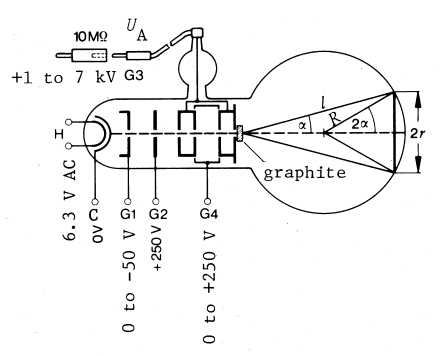
\includegraphics[scale=1.79]{versuchsaufbau.png}
\caption{Aufbau des Versuchs. Quelle: \cite{moodle}}
\label{fig:aufbau}

\end{figure}



\section{Geräteliste}


\begin{table}[H]
\caption{Liste der verwendeten Geräte}
~
\begin{tabular}{l|l}
 & Geräte  \\
\hline
1 & Hauptgerät (siehe Abb.~\ref{fig:aufbau})\\
2 & Paar Helmholtzspulen\\	
3 & Netzgerät\\
4 & Schiebelehre \\
5 & Heizspannungsquelle \\
6 & Multimeter (Fluke 175)
\end{tabular}

\end{table}


\section{Durchführung und Messergebnisse}

\subsection{Beugung an der Graphitprobe}

Zuerst wurde gemäß Skript die Heizspannung eingeschalten und der Kathodenstrom wie im Skript~\cite{moodle} beschrieben auf 0.3~A begrenzt. Die Anodenspannung wurde dann schrittweise erhöht, um den Durchmesser der Ringe messen zu können. Es hat sich in der Praxis gezeigt, dass Werte zwischen 2~kV und 5~kV geeignet sind. Unter 2~kV warem die Ringe sehr schlecht zu erkennen, sodass eine genaue Messung nicht sinnvoll war. Umgekehrt war 4.87~kV der höchste Wert, der bei der Spannung durch technische Limits erreicht werden konnte.


\begin{table}[H]
\caption{Gemessene Durchmesser zweier Beugungsringe bei gegebener Spannung $U$.}
\label{tab:exp1}
\begin{tabular}{r|rr|rr}
$U$ / kV & $d_{\text{innen},1}$ / mm & $d_{\text{aussen},1}$ / mm & $d_{\text{innen},2}$ / mm & $d_{\text{aussen},2}$ / mm \\
\hline
2.25 & 35 & 36 & 56 & 59\\
2.50 & 32 & 35 & 55 & 58\\
2.75 & 31 & 33 & 56 & 57\\
3.00 & 30 & 31 & 49 & 52\\
3.25 & 27 & 29 & 48 & 50\\
3.50 & 24 & 27 & 45 & 48\\
3.75 & 26 & 27 & 45 & 47\\
4.00 & 25 & 26 & 45 & 46\\
4.25 & 21 & 24 & 42 & 44\\
4.50 & 18 & 21 & 40 & 41\\
4.87 & 19 & 21 & 36 & 39\\
\end{tabular}

\end{table}



%
%\begin{figure}[H]
%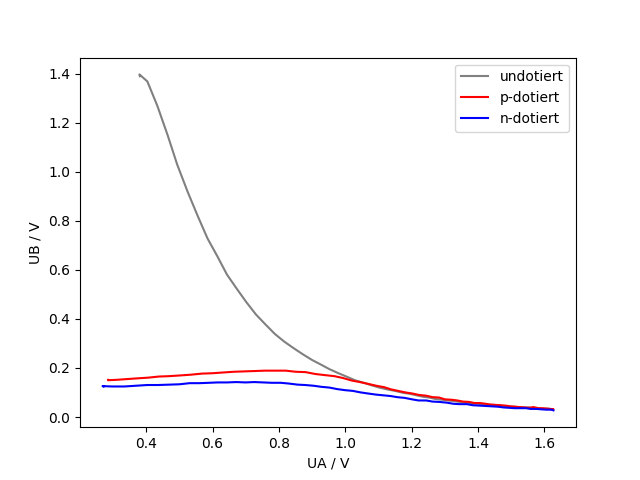
\includegraphics[scale=1.]{data_raw.png}
%\caption{Spannungen wie sie gemessen wurden, wobei UA auf der x-Achse und UB1 auf der y-Achse aufgetragen wird.}
%\label{fig:data_raw}
%\end{figure}

%
%\begin{figure}[H]
%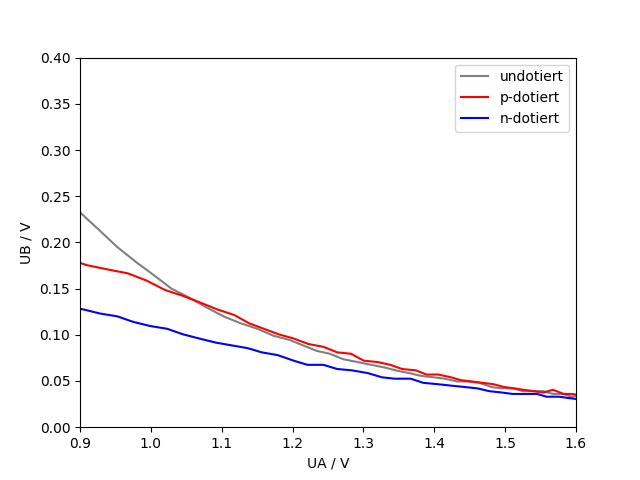
\includegraphics[scale=1.]{data_scaled.png}
%\caption{Dieselben Spannungen wie Grafik~\ref{fig:data_raw}, mit eingeschränktem Wertebereich.}
%\label{fig:data_scaled}
%\end{figure}



\subsection{Bahn im homogenen Magnetfeld}
Hier wurden 2 Messreihen jeweils mit 2~kV und 4~kV aufgenommen. 	Dann wurde die Abweichung in Abhängigkeit von der Stromstärke notiert. Um ein genaueres Ergebnis zu erhalten, wurde der Strom umgepolt und die Abweichung \underline{in beide Richtungen} bestimmt. Durch die Messung der doppelten Abweichung erhält man ein genaueres Ergebnis. Allerdings muss das gemessene Ergebnis für weitere Berechnungen durch 2 dividiert werden.

\begin{table}[H]
\caption{Messung der Elektronenabweichung im homogenen Magnetfeld. Dabei beschreibt $I_1$ und $d_1$ die Abweichung bei einer Spannung von $2~$kV und $I_2$ und $d_2$ die Abweichung bei einer Spannung von $4~$kV.}
\label{tab:exp2_messung}
\begin{tabular}{r|r}
$I_1$ / mA & $d_1$ / mm \\
\hline
25.28 & 14\\
41.86 & 20\\
51.94 & 21\\
60.25 & 26\\
78.50 & 33\\
98.40 & 38\\
120.90 & 51\\
138.40 & 58\\
162.50 & 64\\
182.60 & 72\\
194.80 & 77\\
\end{tabular}\quad\quad\quad\begin{tabular}{r|r}
$I_2$ / mA & $d_2$ / mm \\
\hline
23.95 & 8\\
50.97 & 15\\
75.80 & 23\\
101.90 & 29\\
128.00 & 38\\
147.70 & 45\\
176.10 & 52\\
202.90 & 61\\
223.70 & 72\\
253.10 & 73\\
272.40 & 77\\
\end{tabular}

\end{table}




\section{Auswertung}

\subsection{Beugung an der Graphitprobe}

Es wurde nun der Mittelwert aus den jeweiligen Innen- und Außendurchmesser berechnet und zusätzlich mit Gleichung~\ref{eq:lambda} die Wellenlänge zur jeweiligen Spannung berechnet. Die Ergebnisse sind in Tabelle~\ref{tab:exp1_auswertung} zu finden.



\begin{table}[H]
\caption{Mittelwerte der jeweiligen Innen- und Außendurchmesser und die Wellenlänge zur jeweiligen Spannung.}
\label{tab:exp1_auswertung}
\begin{tabular}{r|rrr}
$U$ / kV & $d_1$ / mm & $d_2$ / mm  & $\lambda$ / pm \\
\hline
2.25 & 35.5 & 57.5 & 25.86\\
2.50 & 33.5 & 56.5 & 24.53\\
2.75 & 32.0 & 56.5 & 23.39\\
3.00 & 30.5 & 50.5 & 22.39\\
3.25 & 28.0 & 49.0 & 21.51\\
3.50 & 25.5 & 46.5 & 20.73\\
3.75 & 26.5 & 46.0 & 20.03\\
4.00 & 25.5 & 45.5 & 19.39\\
4.25 & 22.5 & 43.0 & 18.81\\
4.50 & 19.5 & 40.5 & 18.28\\
4.87 & 20.0 & 37.5 & 17.57\\
\end{tabular}

\end{table}



Durch Anwendung von Formel~\eqref{eq:gitterabstand} kann der entsprechende Gitterabstand zu einem Ring ausgerechnet werden. Die Ergebnisse sind in folgender Tabelle zusammengestellt.


\begin{table}[H]
\caption{Gitterabstände zu den Ringen.}
\label{tab:exp1_result}
\begin{tabular}{r|rr}
$\lambda$ / pm & $D_1$ / pm & $D_2$ / pm  \\
\hline
25.86 & 196.6 & 121.4\\
24.53 & 197.7 & 117.2\\
23.39 & 197.3 & 111.8\\
22.39 & 198.2 & 119.7\\
21.51 & 207.4 & 118.5\\
20.73 & 219.5 & 120.4\\
20.03 & 204.1 & 117.6\\
19.39 & 205.3 & 115.1\\
18.81 & 225.8 & 118.1\\
18.28 & 253.1 & 121.9\\
17.57 & 237.3 & 126.5\\
\end{tabular}

\end{table}

Durch Bildung des Mittelwertes und der Standardabweichung kann man nun die Gitterabstände berechnen.
\begin{align}
D_1 &= \left(212.94 \pm 17.94\right)~\text{pm}\\
D_2 &= \left(118.93 \pm 3.66\right)~\text{pm}
\label{eq:gitterabst_result}
\end{align}



\subsection{Bahn im homogenen Magnetfeld}
Zuerst muss der Bahnradius mit Gleichung~\eqref{eq:radius} bestimmt werden. Zusätzlich muss die Abweichung aus \ref{tab:exp2_messung} halbiert werden, da die doppelte Abweichung gemessen wurde. Es folgt Tabelle~\ref{tab:exp2_radien}.

\begin{table}[H]
\caption{Krümmungsradien zu den Abweichungen. $I_1$ und $s_1$ sind der Strom und die dazugehörige Abweichung für $U_1=2~$kV. Zusätzlich ist $r_1$ der Krümmungsradius für die jeweilige Abweichung. Analog gilt das für $I_2$, $s_2$ und $r_2$ für $U_2=4$~kV.}
\label{tab:exp2_radien}
\begin{tabular}{r|rrr}
$I_1$ / mA & $s_1$ / mm & $r_1$ / mm & $B_1$ / $\mu$T \\
\hline
25.28 & 7.0 & 1300 & 107\\
41.86 & 10.0 & 909 & 177\\
51.94 & 10.5 & 865 & 220\\
60.25 & 13.0 & 698 & 255\\
78.50 & 16.5 & 548 & 332\\
98.40 & 19.0 & 475 & 416\\
120.90 & 25.5 & 351 & 512\\
138.40 & 29.0 & 307 & 586\\
162.50 & 32.0 & 277 & 688\\
182.60 & 36.0 & 244 & 773\\
194.80 & 38.5 & 227 & 824\\
\end{tabular}\quad\quad\quad\begin{tabular}{r|rrr}
$I_2$ / mA & $s_2$ / mm & $r_2$ / mm & $B_2$ / $\mu$T \\
\hline
23.95 & 4.0 & 2277 & 101\\
50.97 & 7.5 & 1213 & 216\\
75.80 & 11.5 & 790 & 321\\
101.90 & 14.5 & 625 & 431\\
128.00 & 19.0 & 475 & 542\\
147.70 & 22.5 & 399 & 625\\
176.10 & 26.0 & 344 & 745\\
202.90 & 30.5 & 291 & 859\\
223.70 & 36.0 & 244 & 947\\
253.10 & 36.5 & 240 & 1071\\
272.40 & 38.5 & 227 & 1153\\
\end{tabular}

\end{table}

Gleichung~\eqref{eq:espez} lässt sich zu 
\begin{align*}
B \cdot \sqrt{\frac{e_\text{spez}}{2\cdot U}} = \frac{1}{r}
\end{align*}
umformen. Durch eine Regression kann daraus $e_\text{spez}$ bestimmt werden. Für die entsprechenden Steigungen gilt
\begin{align*}
e_\text{spez} = 2\cdot U \cdot k^2
\end{align*}

Die Regression wurde durchgeführt. Die Regressionsgeraden sind in Abbildung~\ref{fig:regression} zusammengefasst. Die Steigungen der Regression sind
\begin{align*}
k_1 &= 5156~\text{m}^{-1}\cdot \text{T}^{-1} \\
k_2 &= 3972~\text{m}^{-1}\cdot \text{T}^{-1} 
\end{align*}

Daraus lässt sich jetzt die spezifische Elektronenladung $e_\text{spez}$ bestimmen. Daraus folgt für die spezifische Elektronenladung
\begin{align*}
e_{\text{spez},1} &= (-1.064\pm0.114)\cdot 10^{11}~\text{C}\cdot \text{kg}^{-1} \\
e_{\text{spez},2} &= (-2.127\pm0.074)\cdot 10^{11}~\text{C}\cdot \text{kg}^{-1} 
\end{align*}


\begin{figure}[H]
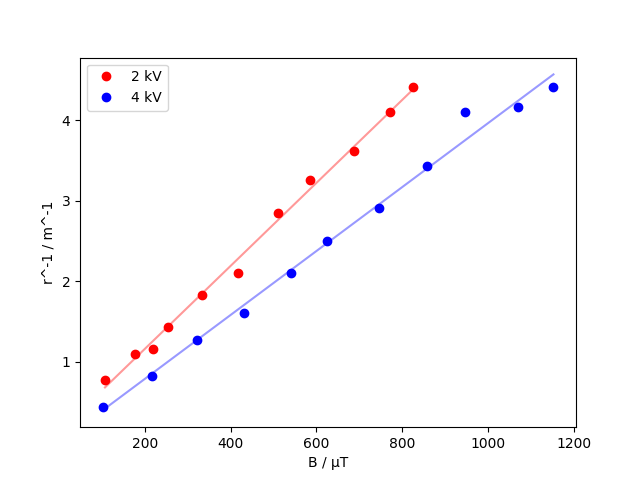
\includegraphics[scale=0.7]{regression.png}
\caption{Regressionsgeraden für den Zusammenhang zwischen $B$ und $1/r$ für jeweils $U_1=2$~kV und $U_2=4$~kV.}
\label{fig:regression}
\end{figure}


\section{Diskussion und Zusammenfassung}
Es zeigt sich, dass die Gitterabstände 
\begin{align*}
D_1 &= \left(212.94 \pm 17.94\right)~\text{pm}\\
D_2 &= \left(118.93 \pm 3.66\right)~\text{pm}
\end{align*}
mit den Werten im Skript \cite{moodle} und Grafik~\ref{fig:gitterabst} übereinstimmen. Lediglich die Abweichung von $D_1$ ist etwas höher. Das liegt daran, dass dieser Gitterabstand durch den inneren Ring gemessen wurde. Da dieser kleiner war, gestaltete sich die Messung schwieriger und ungenauer. 

Die spezifische Ladung kann experimentell bestimmt werden. Ein Wert aus dem Internet ist
\begin{align*}
e_\text{spez} = -1.758~820~010~76(53)\cdot 10^{11}~\text{C}\cdot\text{kg}^{-1}
\end{align*}

In unserem Fall liegt ein Wert darüber und einer darunter. Da könnte man durch Mittelwertbildung eine bessere Näherung erhalten. 

Die Messungenauigkeiten kommen unter anderem von der Ungenauigkeit durch die Messung mit der Schiebelehre. Da die Längen auf einer gewölbten Ebene abzulesen sind, kann bei der Messung eine Ungenauigkeit entstehen.

Die spezifische Elektronenladung sollte gemäß Angabe durch Regression bestimmt werden. Alternativ hätte man auch in Tabelle~\ref{tab:exp2_radien} mit Formel~\eqref{eq:espez} die spezifische Elektronenladung bestimmen können. Hierbei erhält man $-1.27\cdot 10^{11}~\text{C}\cdot\text{kg}^{-1}$ bzw. $-1.26\cdot 10^{11}~\text{C}\cdot\text{kg}^{-1}$.


\begin{thebibliography}{9}
\bibitem{moodle} M. Ramsey: Skript zu Elektronenbeugung aus dem Moodle der Karl-Franzens Universität, Institut für Physik, 28.05.2021.
\bibitem{messmethoden}  R. Dämon: Einführung in die physikalischen Messmethoden, Graz 2016.
\bibitem{AKT}  J. Winkler: Unterlagen (Mitschrift) zur Atom-, Kern und Teilchenphysik Vorlesung des Wintersemesters 2020, Vorlesung gehalten von M. Schultze, Graz 2020.
\bibitem{demtroeder} W. Demtröder: \emph{Experimentalphysik 2 - Elektrizität  und Optik}, 7. Auflage, 2017.
\bibitem{python} Python-Skript zur Berechnung der Daten, zur Visualisierung und zum Generieren von \LaTeX-Code für diesen Bericht.
\bibitem{wikipedia} \url{https://de.wikipedia.org/wiki/Spezifische_Ladung}, 28.05.2021.
\end{thebibliography}


\newpage 
%\appendix
%\section{Python Skript}



\definecolor{commentgreen}{RGB}{2,112,10}
\definecolor{eminence}{RGB}{108,48,130}
\definecolor{weborange}{RGB}{255,165,0}
\definecolor{frenchplum}{RGB}{129,20,83}

\lstdefinelanguage{python}{
    morekeywords={def, for, range, abs, return},
    otherkeywords={<-,->, |>, \%\{, \}, \{, \, (, )},
    sensitive=true,
    morecomment=[l]{\#},
    morecomment=[n]{/*}{*/},
    morecomment=[s][\color{purple}]{:}{\ },
    morestring=[s][\color{orange}]"",
    commentstyle=\color{commentgreen},
    keywordstyle=\color{eminence},
    stringstyle=\color{red},
	basicstyle=\ttfamily,
	breaklines,
	showstringspaces=false,
	frame=tb
}
%\lstinputlisting[language=Python,captionpos=b, label=lst:test,caption={Auswertung}]{script.py}

%\lstinputlisting[language=Python,captionpos=b, label=lst:test,caption={Bessel Auswertung}]{generate_numbers_bessel.py}



\end{document}